% This file is 'adgr.tex'
%
% Copyright (c) 2007 Axel Tetzlaff and Timo Hübel

\documentclass[a4paper,twocolumn,abstracton]{scrartcl}
\usepackage[utf8]{inputenc}
\usepackage{ngerman}
\usepackage{graphicx}
\usepackage{hyperref}
\usepackage[numbers]{natbib}

\addtokomafont{caption}{\small\itshape}
\setkomafont{captionlabel}{\bfseries}
\setcapindent{1em}

\clubpenalty = 999
\widowpenalty = 999

\begin{document}
\titlehead{\textsc{Fachhochschule Wedel\\Wintersemester 2006/2007}}
\subject{Advanced Graphics}
\title{Implementation eines Raytracers mit Photon Mapping}
\author{Axel Tetzlaff \and Timo Hübel}
\date{16. Februar 2007}
\maketitle

\begin{abstract}
\textit{
Anhand einer beispielhaften Implementation wird im Folgenden das Photon Mapping Verfahren genauer vorgestellt. Es handelt sich dabei um einen von Henrik W. Jensen im Jahre 1995 vorgestellten Ansatz, die Berechnung der globalen Beleuchtung in computergenerierten Bildern zu beschleunigen. Die Methode beruht dabei auf der Idee, die Verteilung des Lichtes innerhalb einer Szene in einer seperaten Datenstruktur zu speichern und dann während der Generierung des Bildes zur korrekten Beleuchtungsberechnung einzusetzen.
}
\end{abstract}

\section{Einleitung}
Die Herausforderung in der Erzeugung realistischer Bilder mit Hilfe des Computers, liegt in der Berechnung der globalen Lichtverteilung innerhalb einer Szene. Da eine Oberfläche in der realen Welt hauptsächlich indirekt beleuchtet wird, das einfallende Licht also mindestens einmal von einer anderen Oberfläche reflektiert wird, bedeutet dies einen hohen Rechenaufwand. Unter der Annahme, dass prinzpiell jede Fläche auf diese Weise mit allen anderen Fläche interagieren kann, ergibt sich eine Komplexität von $O(N^2)$ Interaktionen bei $N$ Flächen. Man spricht dabei auch vom \emph{global illumination} Problem \citep{Shirley2005}. Traditionell findet das Verfahren eher Verwendung im Bereich des Offline-Rendering und ist inzwischen in nahezu jedem bekannten Renderer integriert \citep{Wikipedia2007a}. In Echtzeitanwendungen wird die globale Beleuchtung in der Regel mit dem sogenannten \emph{ambient light} approximert \citep{Shreiner2004}. Mit der Verfügbarkeit von programmierbarer Grafikhardware ist aber auch die Anwendung von Photon Mapping in Echtzeitanwendungen möglich \citep{Purcell2003, Larsen2004}.

\section{Photon Mapping}
Wie bei anderen Verfahren zur Berechnung der globalen Beleuchtung in einer Szene ist es auch beim Photon Mapping das Ziel, die \emph{rendering equation} von Kajiya zu lösen \citep{Jensen2001}.

Die Motivation zur Entwicklung des Photon Mappings ergab sich primär aus den Unzulänglichkeiten der vorhandenen Verfahren. Monte Carlo Raytracing ist zwar in der Lage, alle Effekte der globalen Beleuchtung zu berechnen und kann auch mit beliebigen Geometrien sowie BRDFs umgehen, ist aber nicht sonderlich effizient und die Ergebnisse leiden unter Rauschartefakten. Das Radiosity Verfahren hingegen ist zwar schneller, hat aber aufgrund der notwendigen Mesh Generierung Probleme mit der Geometrie und der BRDF bei spekularen Oberflächen \citep{Jensen2001}.

\subsection{Konzept}
Aufgrund der Anforderungen an das Photon Mapping scheint die Erweiterung des Monte Carlo Raytracing naheliegend. Dieses bietet alle gewünschten Eigenschaften und muss nur hinsichtlich der Performanz und des Bildrauschens optimiert werden. Dazu wird beim Photon Mapping die Tatsache ausgenutzt, dass sich die Strahldichte (die spezifische Intensität) über größere Regionen einer Szene in der Regel sehr gleichmäßig verteilt. Es erscheint also sinnvoll, in diesen Fällen die Informationen über die Beleuchtung zu speichern und wiederzuverwenden, anstelle sie bei jedem Auftreffen eines Strahls auf eine Fläche wie beim Monte Carlo Verfahren neu zu berechnen. Dabei soll jedoch die Unabhängigkeit von der Repräsentation der Geometrie gewährleistet sein. Dazu entwickelte Henrik W. Jensen die folgenden Ideen: Entkopplung der Darstellung der Beleuchtung von der Geometrie und Speicherung der Informationen über die Beleuchtung als Punkte in einer globalen Datenstruktur \citep{Jensen2001}.

Die Idee des Algorithmus lässt sich also in Kurzform folgendermaßen erklären: Es wird standardmäßiges Monte Carlo Raytracing mit folgendem Unterschied genutzt: Statt der rekursiven Weiterverfolgung der Strahlen nach einer Reflektion wird die von einem Punkt ausgehende Strahlung mit der Hilfe der Photon Map berechnet. Wie genau die Speicherung realisiert ist und aus den gespeicherten Photonen die ausgehende Strahlung berechnet werden kann, wird in den folgenden Abschnitten erläutert.

\subsection{Speichern der Photonen}
In fast allen Programmen stellt der Prozess des Suchens die größte Herausforderung dar, nimmt also einen Großteil der Laufzeit in Anspruch \citep{Knuth1997}. Dies ist beim Photon Mapping nicht anders, da während der Erzeugung des Bildes intensiv nach Photonen in der Photon Map gesucht wird. Daher stellt die Speicherung der Photonen den kritischen Teil einer Implementation des Photon Mapping Verfahrens dar.

\begin{figure}[htb]
\centering
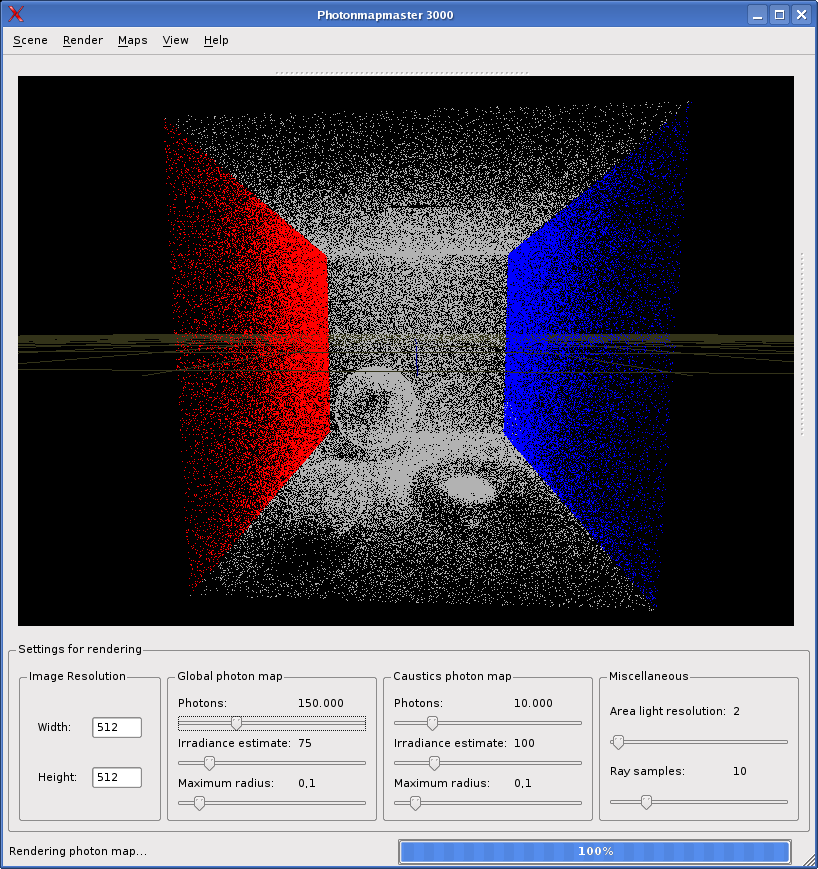
\includegraphics[width=0.48\textwidth]{img/global}
\caption{Verteilung von 150.000 Photonen in einer Photon Map}
\label{fig:global}
\end{figure}

Die einzelnen Photonen werden als Punkte im dreidimensionalen Raum in einer seperaten Datenstruktur abgelegt. Um nun zu einem beliebigen Punkt in der Szene eine Anzahl von Photonen zu Suchen, muss ein entsprechend schneller Zugriff in Abhängigkeit von drei Dimensionen möglich sein. Henrik W. Jensen empfiehlt dazu einen \emph{Kd-Tree} zu benutzen. Es handelt sich dabei um einen k-dimensionalen, balancierten (ausgeglichenen) binären Suchbaum. Ein solcher Baum wird auch \emph{AVL-Baum} genannt \citep{Duden2001a, Duden2001b}. Der Baum arbeitet mit einer Raumaufteilung durch Ebenen orthogonal zu den Koordinatenaxen und ermöglicht es, entsprechende Bereichsanfragen durchzuführen. Diese lassen sich in Abhängikeit der gewünschten Antwortgröße $a$ in $O(n^{1-\frac{1}{k}}+a)$ durchführen \citep{Wikipedia2007b}.

\subsection{Photon Tracing}
Als \emph{Photon Tracing} bezeichnet man den Vorgang des Verfolgens der Wege, auf denen die von einer Lichtquelle ausgesendeten Photonen durch die Szene verlaufen. Dieses Verfahren wird zum Aufbau der Photon Map genutzt. Die Photonen werden dazu an den Lichtquellen erzeugt. Dies ist mit verschiedenen Arten von Lichtquellen möglich, z.B. Punktlichtquellen, gerichtete Lichtquellen oder flächige Lichtquellen. In der Regel werden großere Anzahlen an Photonen erzeugt. Es wird dann die Leistung (Helligkeit) einer Lichtquelle durch die Anzahl der für diese Lichtquelle erzeugten Photonen geteilt. Jedes für diese Lichtquelle emittierte Photon trägt dann einen solchen Teil der Leistung. Dabei ist es wichtig, dass die Leistung proportional zu der Anzahl an emittierten Photonen ist, nicht jedoch zu der Anzahl tatsächlich in der Photon Map gespeicherten Photonen.

Wenn ein Photon emittiert wird, dann erfolgt die Verfolgung seines Weges genau so wie die Verfolgung eines Strahls beim \emph{Raytracing} auf seinem Weg durch die Szene. Der einzige Unterschied besteht darin, dass ein Photon Leistung transportiert, während der Strahl beim Raytracing Intensitäten "`aufsammelt"'. Wenn ein Photon auf ein Object trifft, dann wird es entweder reflektiert, transmittiert oder absorbiert. Diese Entscheidung wird aufgrund der Materialeigenschaften der Objektoberfläche getroffen.

\minisec{Spekulare Reflektion}
Wenn ein Photon ein spiegelnde Oberfläche trifft, dann wird ein neues Photon in gespiegelter Richtung reflektiert. Mit der Normale $\vec{n}$ der Oberfläche und der Richtung $\vec{w'}$ des eintreffenden Photons lässt sich die reflektierte Richtung $\vec{w}$ berechnen wie folgt \citep{Jensen2001, Shirley2005}:
\begin{displaymath}
\vec{w} = 2(\vec{n} \cdot \vec{w'})\vec{n} - \vec{w'}
\end{displaymath}
Die transportierte Leistung des reflektierten Photons wird mit der Reflektivität der Oberfläche skaliert, es sei denn, es wird Russian Roulette verwendet.

\minisec{Diffuse Reflektion}
Wenn ein Photon auf eine diffuse Oberfläche trifft, dann wird es in der Photon Map gespeichert. Die Richtung des diffus reflektierten Photons wird berechnet, indem ein zufälliger Punkt auf der Hemisphäre über dem Schnittpunkt mit der Oberfläche gewählt wird. Die transportierte Leistung wird mit der diffusen Reflektivität der Oberfläche skaliert, es sei denn, Russian Roulette wird verwendet.

\minisec{Russian Roulette}
Um die Berechnung zu beschleunigen, kann eine Technik mit dem Namen \emph{Russian Roulette} eingesetzt werden. Es handelt sich dabei um eine stochastische Methode, mit deren Hilfe unwichtige Photonen entfernt und die Berechnung somit auf die wichtigen Photonen konzentriert werden kann. Ebenfalls wird auf diese Weise sichergestellt, dass die gespeicherten Photonen ähnliche Leistungen tragen \citep{Jensen2001}.

Russian Roulette beruht auf der Idee, dass durch die Auswahl über eine Wahrscheinlichkeitsverteilung, mit weniger Rechenaufwand trotzdem ein korrektes Ergebnis erzielt werden kann. So wird z.B. anhand einer Zufallsverteilung und einer Reflektivitäts-Wahrscheinlichkeit als Materialeigenschaft der Oberfläche des Objekts für ein Photon über spekulare Reflektion, diffuse Reflektion oder Absorption entschieden.

\subsection{Der Radiance Estimate}
Anhand einer gegebenen Photon Map können verschiedene Stastiken über die Beleuchtung innerhalb der Szene berechnet werden. So kann z.B. aus der Dichte der Photonen in einer Region abgeleitet werden, wieviel Licht diesen Bereich erreicht. Die wichtigste Eigenschaft, welche mit Hilfe der Photon Map berechnet werden kann, ist jedoch der \emph{Radiance Estimate}, also eine Näherung der reflektierten Strahlung an einem beliebigen Punkt in der Geometrie \citep{Jensen2001}.

Ein einzelnes Photon in der Photon Map repräsentiert den einfallenden Srahlungsfluss an einem konkreten Punkt. Daraus lässt sich schließen, dass die entsprechende Region in der Geometrie entweder direkt oder indirekt von einer Lichtquelle beleuchtet wird. Allerdings gibt ein einzelnes Photon noch keine Auskunft über die Beleuchtungsstärke in dieser Region. Diese kann erst anhand die Dichte der Photonen in der Region bestimmt werden.

Für das Rendering eines Bildes ist jedoch nicht die Beleuchtungsstärke (also einfallendes Licht) in einer Region ausschlaggebend, sondern es wird die reflektierte Strahlung an einem Punkt benötigt. Diese lässt sich jedoch aus der Beleuchtungsstärke (und somit anhand der Photonen in der Photon Map) berechnen. Die reflektierte Strahlungsdichte $L_r$ and der Stelle $x$ in Richtung $\vec{\omega}$ lässt sich, abgeleitet aus der \emph{rendering equation}, folgendermaßen berechnen \citep{Jensen2001, Shirley2005}:
\begin{displaymath}
L_r(x,\vec{\omega}) = \int\limits_{\Omega_x} f_r(x,\vec{\omega}',\vec{\omega}) L_i(x,\vec{\omega}') (\vec{n}_x \cdot \vec{\omega}') d\vec{\omega}'
\end{displaymath}
Dabei sei $\Omega_x$ die Hemisphäre der eingehenden Richtungen und $f_r$ die BRDF am Punkt $x$. Darüber hinaus bezeichnet $L_i$ die einfallende Strahlungsdichte, welche anhand des einfallenden Strahlungsfluss aus der Photon Map berechnet werden kann. Dazu wird der Strahlungsfluss über eine Anzahl $n$ an Photonen innerhalb eines bestimmten Radius am Punkt $x$ approximiert. Unter der Annahme, dass die Oberfläche am Punkt $x$, lokal gesehen, einer Ebene entspricht, ergibt sich folgende Gleichung zur Berechnung der reflektierten Strahlungsdichte an einem beliebigen Punkt $x$ der Szene:
\begin{displaymath}
L_r(x,\vec{\omega})\approx\frac{1}{\pi r^2}\sum\limits_{p=1}^{N}f_r(x,\vec{\omega}_p,\vec{\omega})\Delta\Phi_p(x,\vec{\omega}_p)
\end{displaymath}
Dabei bezeichnet $\vec{\omega}_p$ die Richtung bzw. $\Delta\Phi_p(\vec{\omega}_p)$ die Strahlungsleistung eines Photons $p$. Die Genauigkeit ist dabei Abhängig von der Anzahl an Photonen in der Photon Map sowie der entsprechenden Anzahl an Photonen $N$ in der Formel. Ebenfalls beeinflusst obige Annahme bzgl. der Beschaffenheit der Geometrie zusammen mit deren tatsächlichen Eigenschaften das Ergebnis \citep{Jensen2001}.

Ein Algorithmus zur Implementation dieser Formel kann für ideal diffuse Flächen entscheidend vereinfacht werden. So ist in diesem Falle die Berechnung der BRDF am Punkt $x$ nicht notwendig. Es ist ausreichend, Photonen auszuschließen, welche auf der Rückseite der Oberfläche eintreffen. Dies kann über einen einfachen Vergleich des Punktproduktes zwischen den Richtungen geschehen \citep{Jensen2001}.

\subsection{Visualisierung}
Der Radiance Estimate lässt sich direkt zum Rendern des Bildes verwenden. Es lässt sich zeigen, dass bei ausreichender Anzahl, die Photonen in der Photon Map schon ausreichend sind um die gesamte globale Beleuchtung in einer Szene zu berechnen. Für gute Ergebnisse ist jedoch eine so große Anzahl an Photonen notwendig, dass sich bei praktischer Anwendung kein nennenswerter Laufzeitvorteil gegenüber dem Monta Carlo Raytracing ergibt \citep{Jensen2001}.

\begin{figure}[htb]
\centering
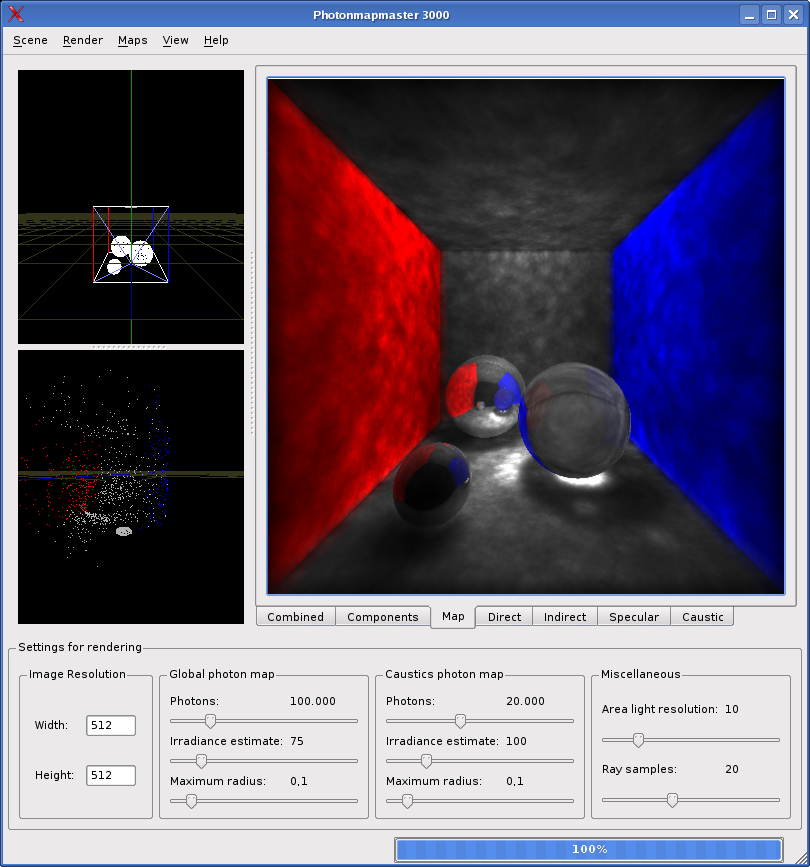
\includegraphics[width=0.48\textwidth]{img/map}
\caption{Visualisierung des Radiance-Estimate}
\label{fig:map}
\end{figure}

In Abbildung \ref{fig:map} ist das Ergebnis eines direkten Rendervorgangs der Photon Map zu sehen. Dazu wird, genauso wie beim Raytracing, ein Strahl vom Augpunkt durch einen Punkt auf der Projektionsfläche in die Szene verfolgt. Am ersten Schnittpunkt mit einer diffusen Oberfläche der Geometrie wird mit Hilfe der Photon Map der Radiance Estimate an dieser Stelle berechnet. Das Ergebnis wird dann direkt als Intensität des Bildpunktes verwendet. In der Abbildung sind sehr gut die wolkenartigen Artefakte zu erkennen, welche sich durch eine entsprechend höhere Anzahl an Photonen aber verringern lassen \citep{Jensen2001}.

\section{Implementation}
Im Folgenden wird unsere konkrete Implementation des Photon Mapping Verfahrens vorgestellt. Der Fokus bei der Entwicklung lag primär auf der verständlichen Darstellung des Verfahrens, daher bietet die Implementation hinsichtlich des effizienten Einsatzes des Photon Mappings noch viel Spielraum für weitere Optimierungen. 

Zunächst erfolgt eine technische Darstellung der Umsetzung des Verfahrens, danach eine allgemeine Beschreibung der Programmfunktionen sowie der Oberfläche.

\subsection{Raytracing}
Der zugrundeliegende Mechanismus zur Erzeugung des Bildes beruht auf dem standardmäßigen \emph{Raytracing}. Um die Intensität eines Pixels im Bild zu berechnen, wird ein Strahl vom Augpunkt aus durch einen Punkt der Projektionsfläche verfolgt, und der erste Schnittpunkt mit einem Objekt der Geometrie berechnet \citep{Purgathofer2002, Shirley2005}. Die eigentliche Berechnung der Intensität kann dann auf verschiedene Arten erfolgen, in unserer Implementation wird dazu die Photon Map verwendet.

Zur Berechnung der Schatten kommen die vom Raytracing bekannten \emph{Schattenstrahlen} zum Einsatz, jedoch mit zusätzlichem Area Sampling über eine flächige Lichtquelle zur Erzeugung von weichen Schattenkanten. Auch die Berechnung der Intensitäten auf spiegelnden bzw. transparenten Oberflächen (spekularer Anteil) erfolgt, wie vom Raytracing gewohnt, durch rekursive Weiterverfolgung der Strahlen in reflektierter bzw. gebrochener Richtung. Die Berechnung der Beleuchtung von diffus reflektierenden Flächen sowie von Caustics (helle Lichterscheinungen durch Bündelung von Lichtstrahlen) erfolgt mit einem \emph{2-Pass Algorithmus}.

\subsection{2-Pass Algorithmus}
Zur Berechnung der Intensität eines Pixels im Bild wird der in \citep{Jensen2001} vorgeschlagene 2-Pass Algorithmus verwendet. Es werden dabei zwei Photon Maps verwendet, eine sogenannte \emph{globale Photon Map}, welche zur Berechnung der indirekten Beleuchtung dient, sowie eine \emph{Caustics Photon Map}, welche speziell für die Darstellung der Caustics benutzt wird. Man spricht von einem 2-Pass Algorithmus, da in einem ersten Schritt die Photon Maps erzeugt werden, während danach in einem zweiten Schritt das eigentliche Bild gerendert wird.

Generell wird die Intensität eines Pixels in vier Anteile aufgeteilt. Dies sind:
\begin{itemize}
 \item \emph{Direkte Beleuchtung} durch eine Lichtquelle
 \item \emph{Indirekte Beleuchtung} durch diffuse Reflektion
 \item \emph{Spekulare Reflektion} bzw. Refraktion an glänzenden bzw. transparenten Oberflächen
 \item \emph{Caustics} aufgrund der Bündelung von Lichtstrahlen
\end{itemize}
Die Gesamtintensität berechnet sich dann aus der Summe dieser Einzelteile. Die indirekte Beleuchtung wird durch die Mittelung mehrerer rekursiv verfolgter Zufallsstrahlen an einem Schnittpunkt berechnet. Allerdings kommt für einen solchen, durch Rekursion erzeugten Strahl bei der nächsten diffusen Reflektion eine andere Art der Berechnung zur Bestimmtung der Intensität zum Einsatz. Zunächst müssen jedoch die Photon Maps erzeugt werden.

\begin{figure}[htb]
\centering
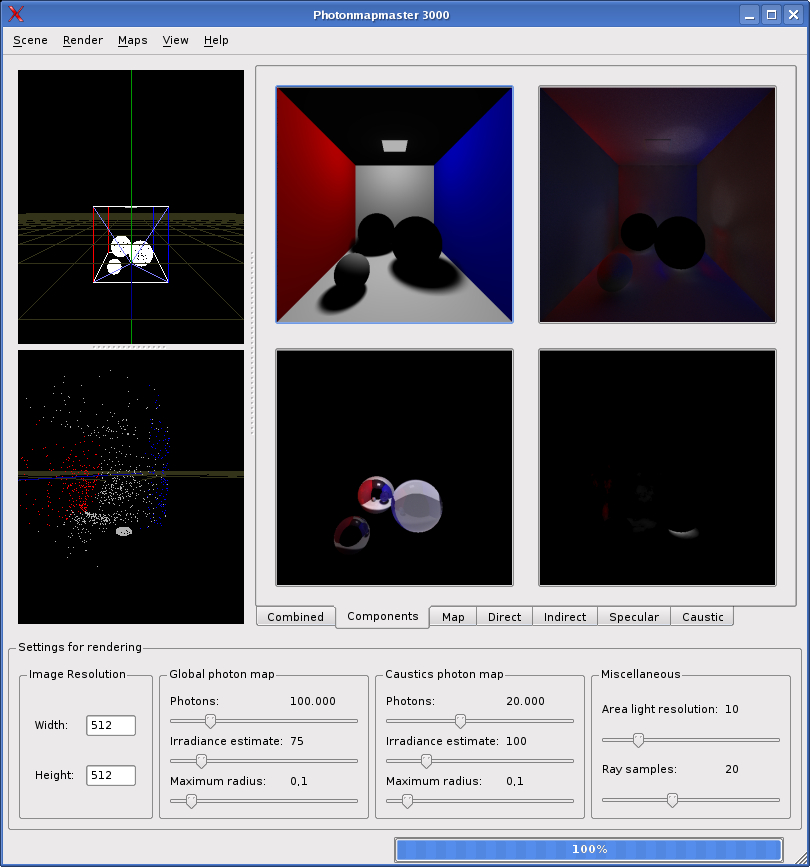
\includegraphics[width=0.48\textwidth]{img/components}
\caption{Die Rendering-Komponenten im 2-Pass Algorithmus}
\label{fig:components}
\end{figure}

\minisec{Erzeugung der Photon Maps}
Die Erzeugung der Photon Maps erfolgt, wie bereits beschrieben, mittels Photon Tracing. Dabei werden die Photonen ausgehend von den Lichtquellen der Szene in die Geometrie geschossen und entsprechend gespeichert. Als Besonderheit werden die Photonen für die Caustics Photon Map nur in die Richtung von Objekten der Szene geschossen, von denen bekannt ist, dass sie eine spiegelnde oder transparente Oberfläche besitzen. Somit können später Caustics von hoher Qualität bei niedriger Photenanzahl in der Caustics Map gerendert werden.

Für die globale Photon Map werden die Photonen jedoch entsprechend der Charakteristik der Lichtquelle in die gesamte Szene geschossen. Diese Map dient später zur Berechnung der gesamten indirekten Beleuchtung, sei es durch diffuse Reflektion, spekulare Reflektion, Transmission oder auch durch Caustics.

\minisec{Rendern des Bildes}
Für jeden Schnittpunkt eines Augstrahls mit der Geometrie, der durch das Raytracing gefunden wurde, muss die Intensität (also die ausgehende/reflektierte Strahlung) berechnet werden. Prinzipiell werden dabei alle vier Anteile einzeln berechnet und dann zusammengesetzt. Die Berechnung kann dabei entweder \emph{genau} oder \emph{ungenau} erfolgen. Die genaue Berechnung findet statt, wenn der Punkt direkt vom Auge (evt. über eine ideale Reflektion oder Transmission) gesehen wird. Die ungenaue Berechnung kommt zum Einsatz, wenn der Punkt aufgrund der rekursiven Verfolgung des Strahls zur Berechnung der indirekten Beleuchtung ermittelt wurde.

\begin{figure}[htb]
\centering
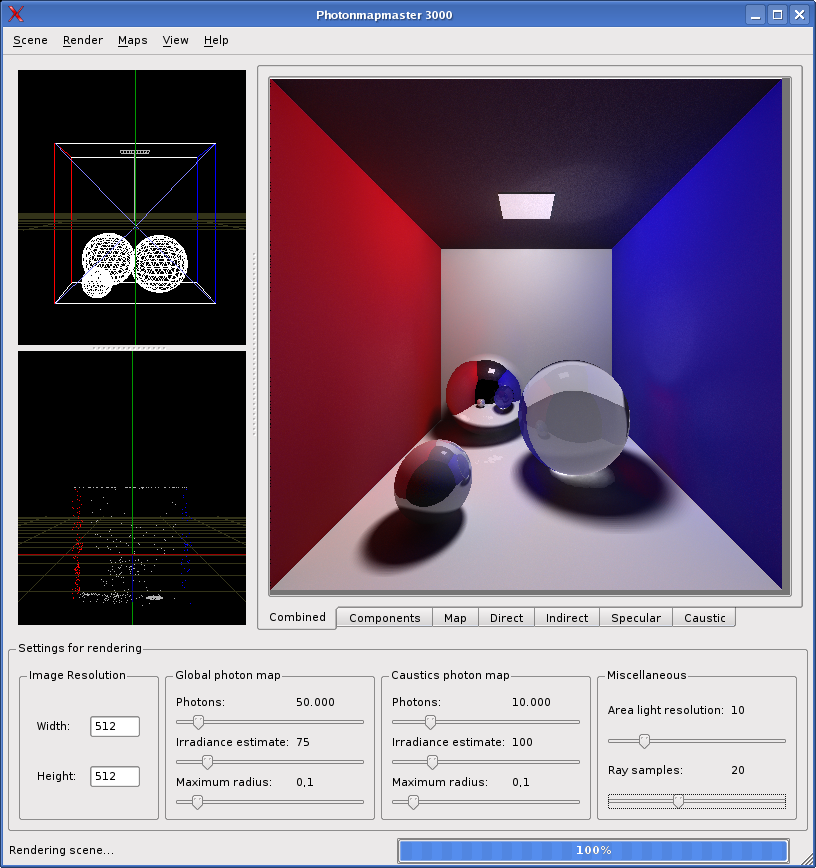
\includegraphics[width=0.48\textwidth]{img/combined}
\caption{Vollständige globale Beleuchtung}
\label{fig:combined}
\end{figure}

Die genaue Berechnung der direkten Beleuchtung erfolgt unter Einsatz klassischer Raytracing Methoden, inkl. der Berechnung der Schatten wie bereits beschrieben. Für die ungenaue Berechnung der direkten Beleuchtung wird der Radiance Estimate mit Hilfe der Photon Map bestimmt.

Für die Berechnung des spekularen Anteils kommt in beiden Fällen dieselbe Methode zum Einsatz. Es wird, wie beim Raytracing üblich, der ideal reflektierte bzw. der ideal transmittierte Strahl rekursiv weiterverfolgt und das Ergebnis des rekursiven Aufrufs zurückgeliefert.

Die genaue Berechnung der Caustics erfolgt anhand des Radiance Estimate aus der Caustics Photon Map. Da bei der Erzeugung viele Photonen für einen beschränkten Teil der Geometrie verwendet wurden, ist die Qualität entsprechend hoch. Die ungenaue Berechnung erfolgt mit Hilfe des Radiance Estimate aus der globalen Photon Map.

Für die genaue Berechnung der indirekten Beleuchtung kommt Monte Carlo Raytracing zum Einsatz, d.h. es werden mehrere, zufällig verteilte Strahlen vom Oberflächenpunkt rekursiv weiterverfolgt und deren Intensitäten gemittelt. Allerdings wird ab der zweiten diffusen Reflektion dann nur noch die ungenaue Methode zur Berechnung eingesetzt, wodurch die maximale Rekursionstiefe auf zwei beschränkt ist. Auch hier erfolgt die ungenaue Berechnung wieder durch den Radiance Estimate aus der globalen Photon Map.

Wichtig für den Algorithmus ist die Tatsache, dass in der globalen Photon Map drei Beleuchtungsarten (direkt, indirekt und Caustics) vereint sind. Wenn also die ungenaue Berechnung der Intensität an einem Punkt in der Szene erfolgt, dann wird nur ein einziges Mal mit Hilfe der globalen Photon Map der Radiance Estimate berechnet. Hieraus ergibt sich, zusammen mit der geringen maximalen Rekursionstiefe gegenüber dem normalen Monte Carlo Raytracing, der Geschwindigkeitsvorteil des Verfahrens.

\subsection{Darstellung und GUI}
Wie in den Abbildungen zu erkennen, glidert sich die Oberfläche in drei Bereiche. Im unteren Bereich lassen sich alle relevanten Parameter zur Erzeugung der Photon Maps sowie für den Rendervorgang einstellen, z.B. die Anzahl an Photonen oder die Auflösung des Bildes. 

Darüber befinden sich auf der linken Seite zwei dreidimensionale Ansichten der Szene, welche sich interaktiv in Echtzeit verändern lassen. In der oberen Ansicht wird die Szene inkl. der Kamera und der Projektionsfläche dargestellt. Darunter befindet sich eine dreidimensionale Ansicht der Photon Map, wobei jeder Punkt einem in der Map gespeicherten Photon entspricht. 

\begin{figure}[htb]
\centering
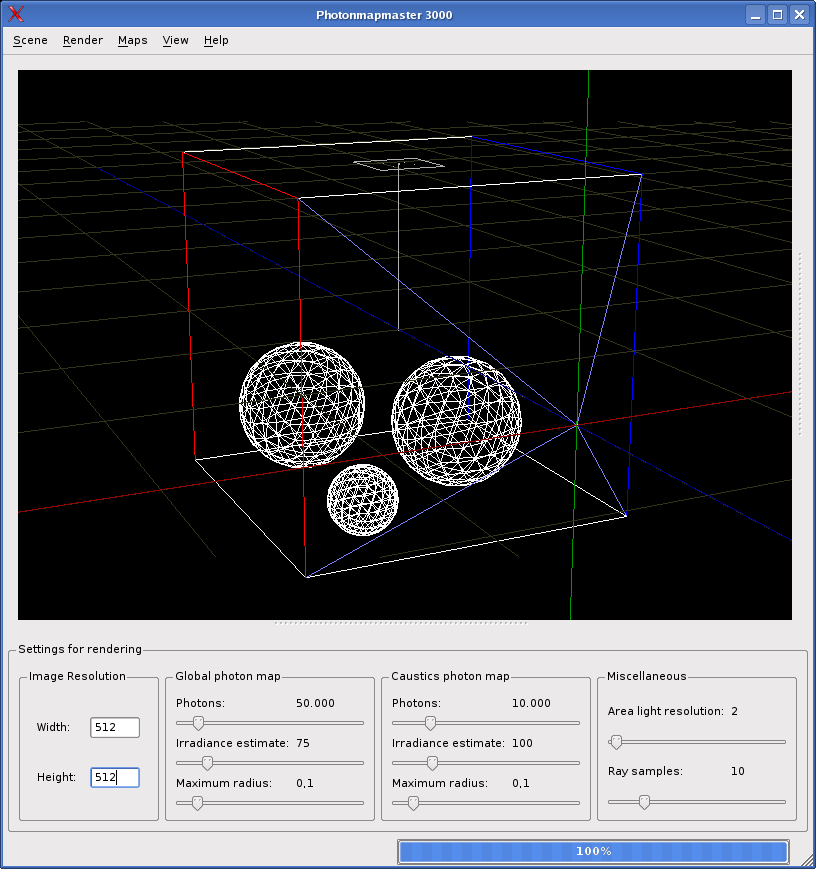
\includegraphics[width=0.48\textwidth]{img/geometry}
\caption{Anzeige der Szene inklusive Kamera mit OpenGL}
\label{fig:geometry}
\end{figure}

Den größten Bereich nimmt die Ansicht des gerenderten Bildes in Anspruch. Es kann über einzelne Tabs zwischen allen vier Komponenten gewählt werden, so ist es möglich, das Gesamtergebnis, aber auch nur den direkten, indirekten oder spekularen Anteil anzuzeigen. Ebenfalls können die Caustics sowie eine Übersicht über alle vier Anteile dargestellt werden. Zusätzlich ist noch eine Anzeige mit dem Ergebnis eines direkten Renderns des Radiance Estimate möglich.

Über das Hauptmenü sind die verschiedenen Aktionen zugänglich. Hier lässt sich eine neue Szene erzeugen, das gerenderte Bild speichern oder es können die Photon Maps erstellt und der Renderingprozess gestartet werden.

\section{Zusammenfassung}
Das Photon Mapping ist ein sehr interessantes Verfahren zur Berechnung der globalen Beleuchtung. Insbesondere die Anlehnung an die Physik des Lichtes erfordert eine andere Denkweise, erleichtert aber andererseits auch das Verständnis. 

Es bleibt jedoch festzuhalten, dass das Photon Mapping allein eigentlich einen naheliegenden Ansatz darstellt. Erst die geschickte Kombination mit Monte Carlo Raytracing bzw. den allgemeinen Mechanismen des Raytracing (ideal transmittierter/reflektierter Strahl, Schattenstrahlen) führt zu sehr effizienten Methoden der Bildgenerierung.

Unsere konkrete Implementation bietet noch weiten Raum für Verbesserungen. So ist z.B. das Materialmodell sehr simpel gehalten und unterstützt nur ideal diffuse, spiegelnde oder durchsichtige Oberflächen. Auch wird mit dem Phong-Modell ein sehr einfaches lokales Beleuchtungsmodell eingesetzt, dies könnte z.B. durch das Schlick Model \citep{Jensen2001} ersetzt werden. Ebenfalls werden mit der Kugel und der Ebene nur zwei sehr elementare Typen an Geometrien unterstützt. Auch hinsichtlich der Laufzeiteffizienz könnte noch vieles optimiert werden, so kommt beispielsweise keine einzige der in \citep{Jensen2001} vorgeschlagenen Optimierungsstrategien zum Einsatz.

%\onecolumn
\bibliographystyle{natdin}
\bibliography{adgr}


\end{document}
